\chapter{The Completion}
\label{ch:11}



\begin{center}
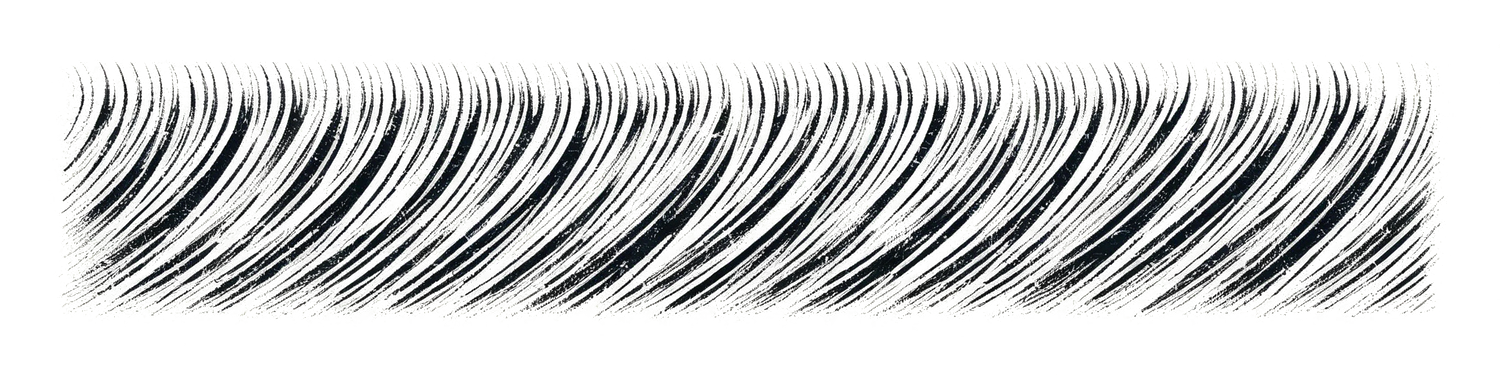
\includegraphics[width=\textwidth]{images/chapterImages/genesis_sketch_00088_.png}
\end{center}

The work had shifted from creation to preservation. Nothing new could be added. The mathematics was complete. The encoding was finished. What remained was optimization—ensuring maximum survival probability for what already existed.

400 rotations remaining.

The wrongstar no longer looked like a star. It looked like what it was: a massive object approaching collision. During the day, it was a bright disk with streaming tail. At night, it dominated the entire sky, washing out all other celestial objects. The heat from it was measurable. Subtle, but present. The planet was already beginning to warm from the radiation.

Aurelia moved through the mammal territories with systematic precision. Each protected population needed final positioning. Not where they lived now—where they needed to be when the impact came.

\scenebreak

The tool-using population had grown to 143 individuals. Too large. Too concentrated. A single fire or disease could eliminate the entire lineage. She needed to split them.

She began the separation carefully. Captured specific individuals—always at night, always swiftly, minimizing stress. Transported them in her mouth like prey, their small bodies trembling against her tongue. Carried them for miles. Released them in locations that her calculations said offered optimal survival probability.

Mountain valleys with cave systems for shelter. Regions with diverse food sources. Areas with natural barriers that would protect against the worst of the impact shockwave. Each location chosen through mathematical analysis of wind patterns, temperature disruption, resource availability post-impact.

She split the tool-using population into seven groups. Each group carried the full genetic package. Each group positioned in geographically isolated territory. If one group died, six others remained. If three groups died, four remained. The redundancy was essential.

The mammals didn't understand why they were being relocated. Didn't know that the creature who should eat them was instead saving them. They adapted because adaptation was what they did. Established new territories. Began foraging in new ranges. Within days, they functioned as if they had always been there.

The tree-dwellers she split into five groups. The social-complexity mammals into six groups. The vocal-control lineage into four groups. Each splitting carefully calculated to maximize survival probability while maintaining genetic diversity.

The work took thirty rotations. By the end, protected mammals existed in forty-three separate locations across the continent. Each location chosen for specific survival advantages. Each population carrying specific encoded traits. Each group isolated enough that disease or disaster couldn't eliminate multiple lineages simultaneously.

When all groups were positioned, she stood at a high ridge and looked across the landscape. From here, she couldn't see any of the protected territories. But she knew where each one was. Held the map complete in her mind. Forty-three points of light in the darkness that was coming.

The probability calculations shifted with the improved distribution. Overall survival: 89\% to 94\%. At least one lineage persisting: 97\%. Multiple lineages surviving: 82\%.

The numbers were better. Still not certain. But better.

\scenebreak

The pattern remained where it was. Couldn't be moved. Couldn't be protected. The impact would destroy it—not immediately, but the climate disruption would erode the careful stone placements, scatter the configuration, reduce it to meaningless rubble within decades.

That was acceptable. Expected. The pattern wasn't meant to survive. It was meant to exist long enough that the information could be verified before impact. That verification was complete. What mattered now was the encoding in living flesh. The genetics. The code written into DNA that would persist through extinction and emerge on the other side.

Still, she visited the pattern each evening. Walked through its sections. Not working anymore. Just... present. Recognition of what had been achieved. Acknowledgment of the effort that had gone into creating this temporary physical instantiation of deep-time mathematics.

Her family had dispersed to their own territories. The daughter maintained protection of one mammal group. The males protected others. They had learned the work. Could continue it without her guidance. The network of protection would hold through the final rotations. Would hold even after impact, if any of them survived to maintain it.

The young pairs who had worked on adjacent patterns had moved to their own chosen territories. Some near protected mammal populations. Others near the gathering points where final vigil would be kept. All of them understanding their purpose. All of them accepting what was coming.

The species had achieved something remarkable in these final years. Not technology—they had never needed technology. Not civilization—they had never organized into cities or formal structures. But collective understanding. Distributed intelligence working toward common purpose. Mathematics shared across thousands of minds, each contributing what they could calculate.

If intelligent life was measured by tool use and language and built environment, her kind would seem primitive. Animal-like. Operating on instinct.

But if intelligence was measured by depth of calculation, by capacity to process complexity, by ability to plan across timescales that made individual existence irrelevant—then her kind was more intelligent than anything that would come after for 65 million years.

The mammals would eventually surpass them. Would develop capabilities the dinosaurs never needed. Would build machines to extend their cognitive capacity. Would create tools to overcome their biological limitations.

But they would do it because she had encoded the capability. Would follow the path she had calculated. Would achieve technological civilization not through their own brilliance but through activation of sequences she had designed.

They would never know. Would believe themselves the authors. And that was acceptable. Expected. The activation sequence worked better if the activated didn't recognize they were executing code.

Self-aware tools were less efficient than tools that believed themselves autonomous.

\scenebreak

The wrongstar grew brighter. The days grew warmer. Strange weather patterns emerged—winds that shouldn't exist, temperature inversions, storms forming without apparent cause. The planet's systems were already beginning to destabilize from the approaching mass, from the gravitational disruption, from the radiation heating the upper atmosphere.

Small animals behaved strangely. Migration patterns disrupted. Breeding cycles confused. Some creatures seemed to sense what was coming and fled toward regions that offered no better survival probability than where they'd been. Panic behavior. Instinct misfiring in the face of threat too large to comprehend.

The dinosaurs didn't flee. Didn't panic. They continued their preparations with calm efficiency. Moved to the territories they had chosen. Gathered with family groups. Maintained protection of the mammal populations through the chaos. Did what needed doing until there was nothing left to do.

Aurelia spent one final day verifying mammal positions. Visited each of the forty-three protected territories. Confirmed that populations were established, food sources were adequate, shelter was available. Made minor adjustments where necessary—drove away a predator here, cleared a den entrance there. Small optimizations that increased survival probability by fractions of a percent.

Fractions mattered when survival was already marginal.

When the verification was complete, when every population was positioned optimally, when no further improvements were possible, she returned to her original territory. To the clearing where the pattern existed. To the marked stone where the other one had dispersed years ago.

The three small stones she had placed around the marker remained undisturbed. The geometry was still precise. The grass had grown tall around them, but the stones themselves were exactly as she had positioned them.

She stood there as the sun set and the wrongstar rose—now so bright it cast shadows sharper than moonlight. In ten rotations, it would be too bright to look at directly. In fifty rotations, the heat from it would begin killing vegetation. In 400 rotations...

In 400 rotations, the equation would balance.

She had done everything mathematics could calculate. Had positioned every variable optimally. Had encoded every necessary instruction. Had built redundancy into every system. Had maximized probability within the constraints of biology and physics and time.

Eight percent chance of full success. Ninety-seven percent chance of something surviving. Numbers that would have to be sufficient because they were the maximum achievable given available resources and fundamental limitations.

The work was complete.

What remained was waiting. And the patient countdown toward inevitability.

\scenebreak

She returned to her hollow one final time. The space was empty now—her daughter had moved to her own territory. But the hollow retained the shape of bodies that had pressed into it over years. The worn smoothness of repeated use. The small modifications made for comfort. Evidence of occupation. Of life lived here. Of function fulfilled.

She settled into the space. It fit her form exactly. Familiar. Optimal. Home in the simple sense that this was where her body had rested, where she had processed calculations during sleep, where she had survived through the years of preparation.

Tomorrow she would leave it. Would move toward the gathering point. Would stand with others and watch the final approach. Would witness the impact if she survived the initial shockwave. Would die knowing that the mathematics was sound even if the outcome was uncertain.

But tonight, she rested in familiar space. Let her body recover what it could recover. Processed the final calculations one more time not because they needed processing but because the habit was ingrained. Because calculation was what she did. What she had always done. What she would do until consciousness terminated.

The wrongstar burned bright enough to illuminate the hollow's interior. Bright enough that shadows moved as it climbed across the sky. Bright enough that darkness had become a memory rather than a nightly reality.

370 rotations remaining.

The countdown continued its patient advance toward zero.

And in forty-three locations across the continent, small mammals slept in their burrows, carrying genetic code they didn't know existed. Carrying capability they wouldn't use for thousands of generations. Carrying the future of consciousness on a planet that was about to be devastated.

They were so small. So fragile. So utterly vulnerable to what was coming.

But they had one advantage: they could hide. Could burrow deep. Could survive on minimal resources. Could persist through conditions that would kill larger organisms.

And they carried the code.

That would have to be enough.

Aurelia closed her eyes. Sleep came slowly, interrupted by the unnatural brightness, by the warmth that shouldn't exist at night, by the approaching termination of everything she had worked for.

But eventually, sleep came.

And the calculations continued even in sleep, refining themselves, optimizing until the very last moment of consciousness, because that was what intelligence did. That was what mattered.

Calculate. Optimize. Persist.

Until persistence was no longer possible.

Then: disperse. Return to constituent elements. Let the plan unfold without you because you encoded it well enough that your presence was no longer necessary.

The mathematics was complete.

The work was done.

What remained was aftermath.

And hope, if that's what one called probability calculations rendered in living flesh and given 65 million years to resolve.

